\input{dfki.defs}

\title[Simulation in Robotics]{Lecture 2 - Simulation of Rigid Body Dynamics}
\author{Julius Martensen}
\date{\today}

\begin{document}


  \frame{\titlepage}

  \section[\Overview]{}
  % Talk about the targets
  % Refer to Christoph and Bernd
  % Give an outline to the lectures

  \frame{\tableofcontents}

  \section{Motivation}
  % Robots are mechatronic systems
  % They are highly interactive
  % The world around them is not

  \section{Rigid Body Dynamics}

    \frame{
      \frametitle{Robots as kinematic chains}
      \begin{figure}
        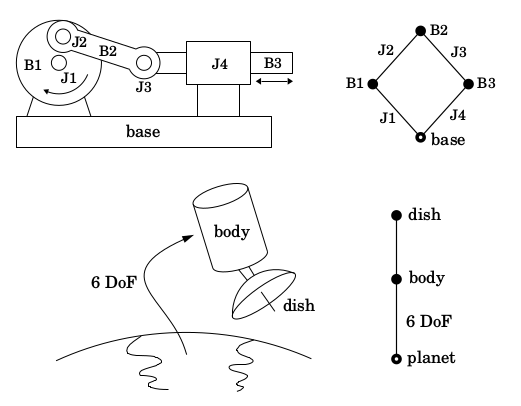
\includegraphics[width = 0.5\textwidth]{./pics/robotic_graph_Featherstone.png}
        \caption{Taken from Featherstone}
      \end{figure}
    }

    \frame{
      \frametitle{Equations of Motion}
      In general, the motion of a mechanical structure can be described as a set of nonlinear differential equations

      \begin{align*}
      M_q \ddot{q} + C(q, \dot{q}) &= \sum \tau
      \end{align}

      Where $M_q \in \mathbb{R}^{m \times m}$ is the generalized inertia matrix,
      $C \in \mathbb{R}^m$ is the vector of centrifugal and gravitational forces
      and $\tau \in \mathbb{R}^m$ are the external forces.

    }

    \frame{
      \frametitle{\textbf{Rigid} Body Movement}
      \begin{figure}
        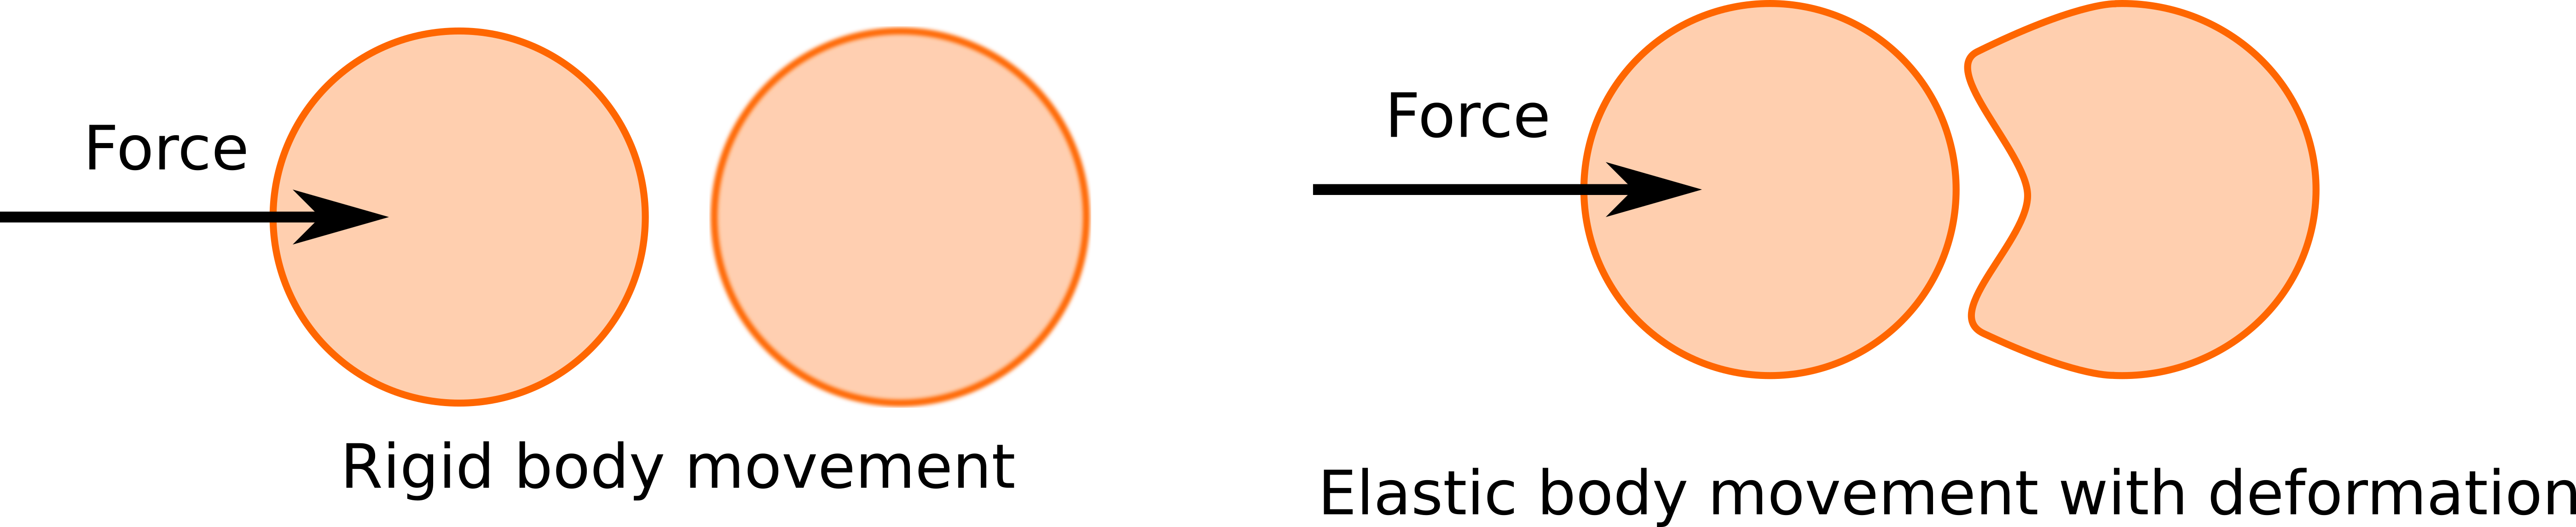
\includegraphics[width = 0.9\textwidth]{./pics/rigid_vs_soft.png}
      \end{figure}

    }

  \section{Constraints}

    \frame{
      \frametitle{A constrained particle}
      \begin{figure}
        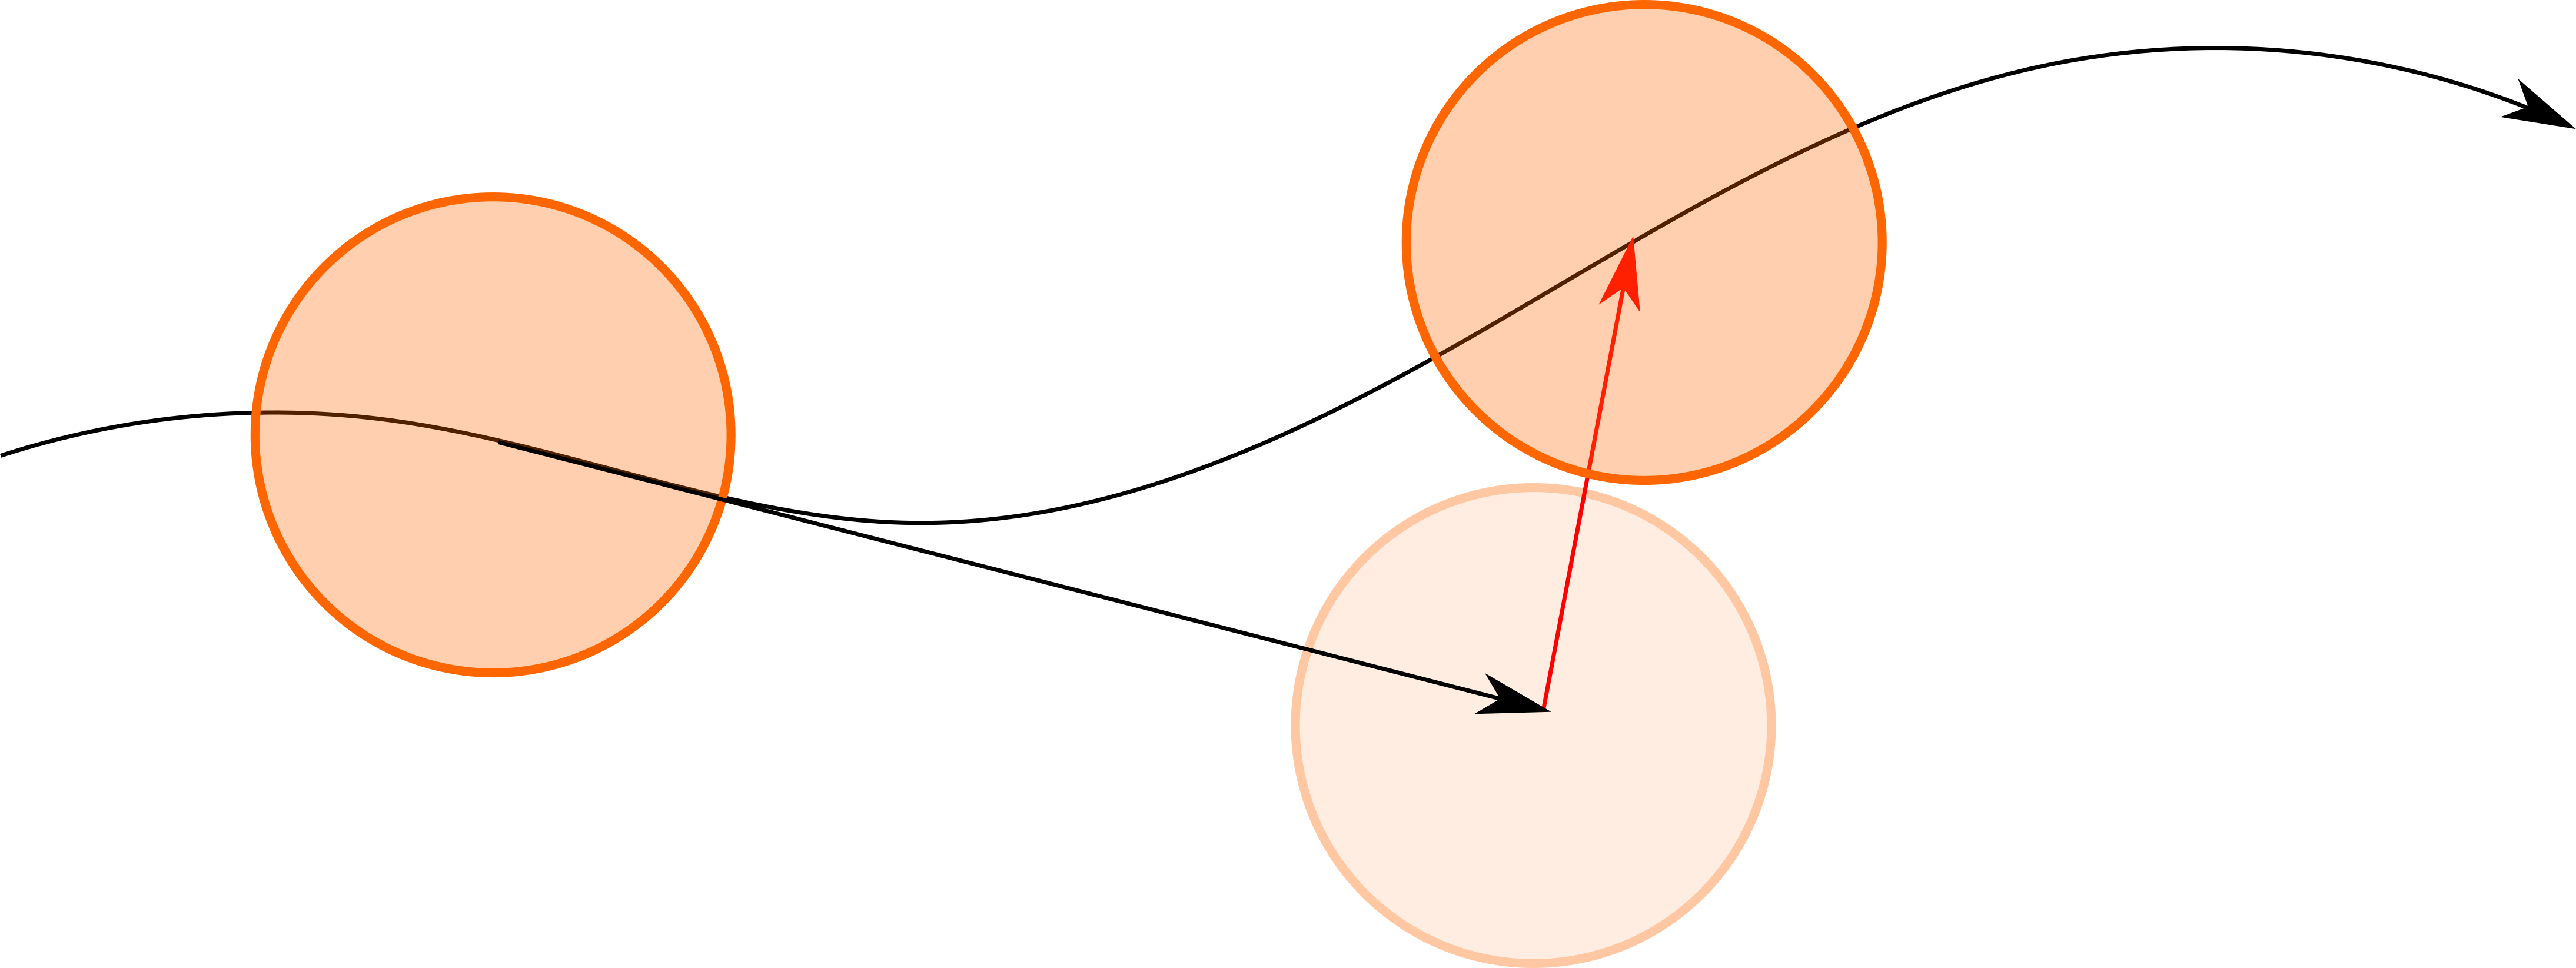
\includegraphics[width = 0.8\textwidth]{./pics/constrains.png}
      \end{figure}

    }

    \frame{
      \frametitle{Description of Constraints}
      The trajectory is constrained via a force which arise due to algebraic constraints:
      \begin{align*}
      Explicit &:~x = f(q) \\
      Implicit &:~g(q) = 0
      \end{align*}
      Which are called holonomic constraints, iff they are only depending on the configuration.\\
    }

    \frame{
      \frametitle{Implementation of Constraints}
      A system under explicit constraints can then be described as:

      \begin{align*}
      M_q \ddot{q} + C(q, \dot{q}) &= \tau + \tau_C \\
      \tau_C &= \frac{df(q)}{dq}^T \lambda \\
            &= J^T \lambda
      \end{align*}

      Which is sufficient to the principle of virtual power.
    }

    \frame{
      \frametitle{Implementation of Constraints}
      Which leads to the following system of equations

      \begin{align*}
      \begin{bmatrix} M_q & J^T \\ J & 0 \end{bmatrix} \begin{bmatrix} \ddot{q} \\ -\lambda \end{bmatrix} &=
      \begin{bmatrix} \tau - C(q,\dot{q}) \\ k \end{bmatrix}
      \end{align*}

      The system is solveable, iff the coefficient Matrix is nonsingular. This is not always the case!
    }

    \frame{
      A common strategy to get the constraint force is to derive the explicit constraint w.r.t. time:

      \begin{align*}
      g(q) &= 0 \\
      \frac{dg}{dt} &= \frac{dg}{dq} \dot{q} = 0 \\
      \frac{d^2g}{dt^2} &= \frac{d}{dt}\left[\frac{dg}{dq} \dot{q} \right]~= ... + \frac{dg}{dq} \ddot{q} = 0
      \end{align*}

      And to solve for $\ddot{q}$.
    }

    \frame{
      This may lead to an increasing error, since we have a numeric precision on acceleration level!
      To compensate, most of the time a controller is implemented based on [BAUMGARTE].
      % Reference to last lecture!
      \begin{figure}
        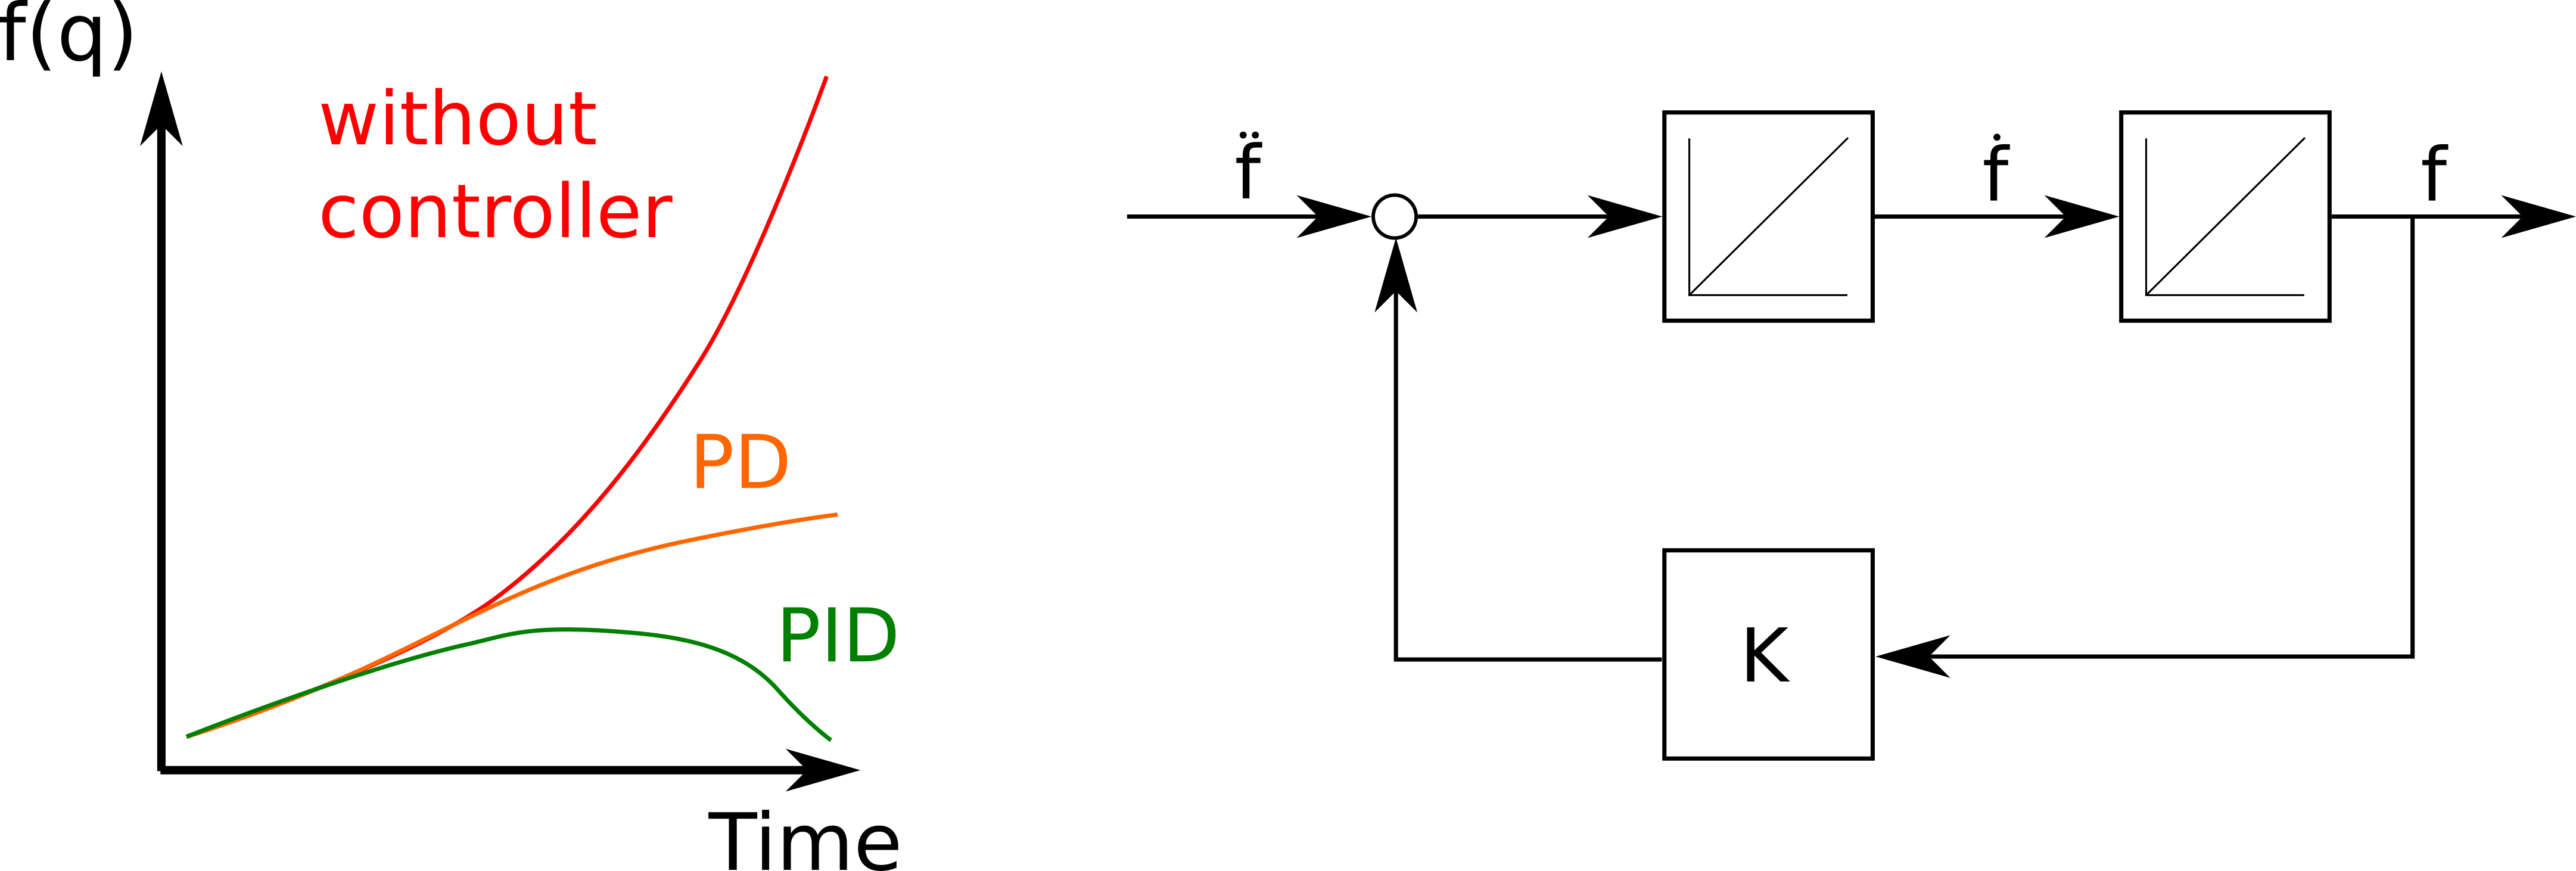
\includegraphics[width = 0.9\textwidth]{./pics/baumgarte.png}
      \end{figure}
    }

    \frame{
      \frametitle{Caveats}
      \begin{itemize}
        \item<1->The controller parameter can often be adjusted within simulation software.
        \item<2-> These techniques reduces the error, but changes the forces in the system.
        \item<3-> A change in the parameter set can change the whole simulation result!
      \end{itemize}

    }
  \section{Collisions and Friction}

    \frame{
      \frametitle{Collisions}
      \begin{figure}
        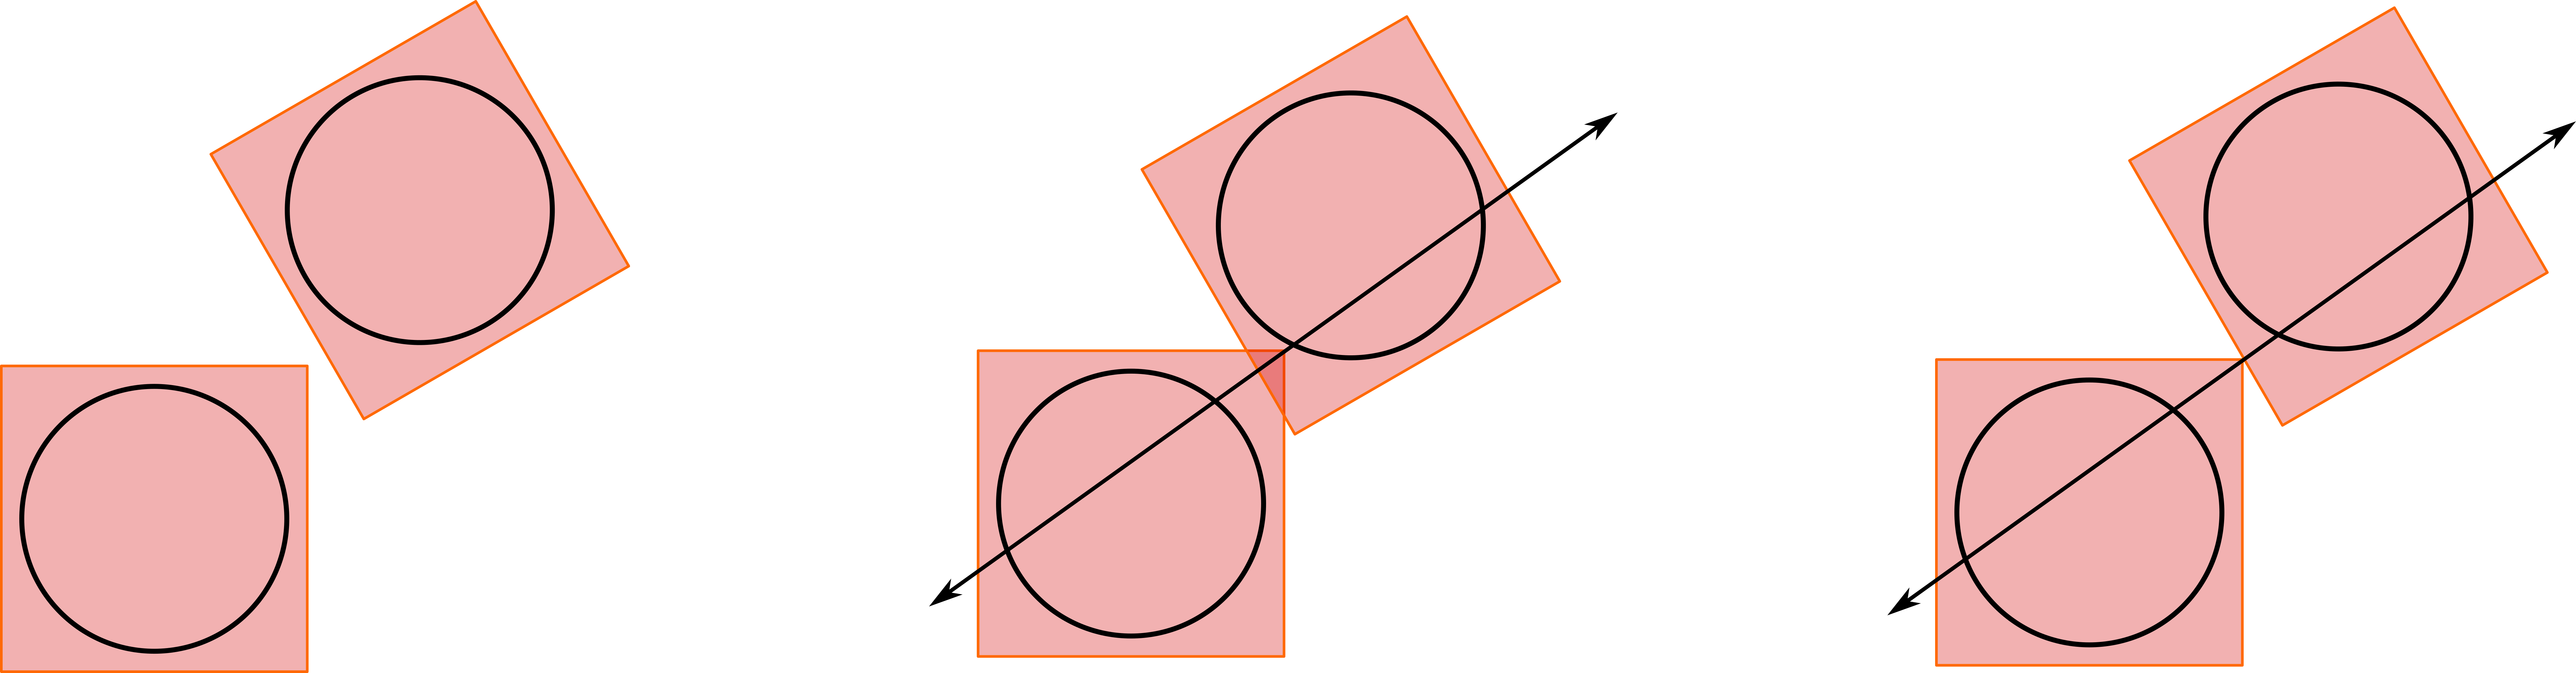
\includegraphics[width = 0.9\textwidth]{./pics/collision_h.png}
      \end{figure}
    }

    \frame{
      \frametitle{Implementation of Collisions}
      \begin{column}{0.5\textwidth}
      \begin{figure}
        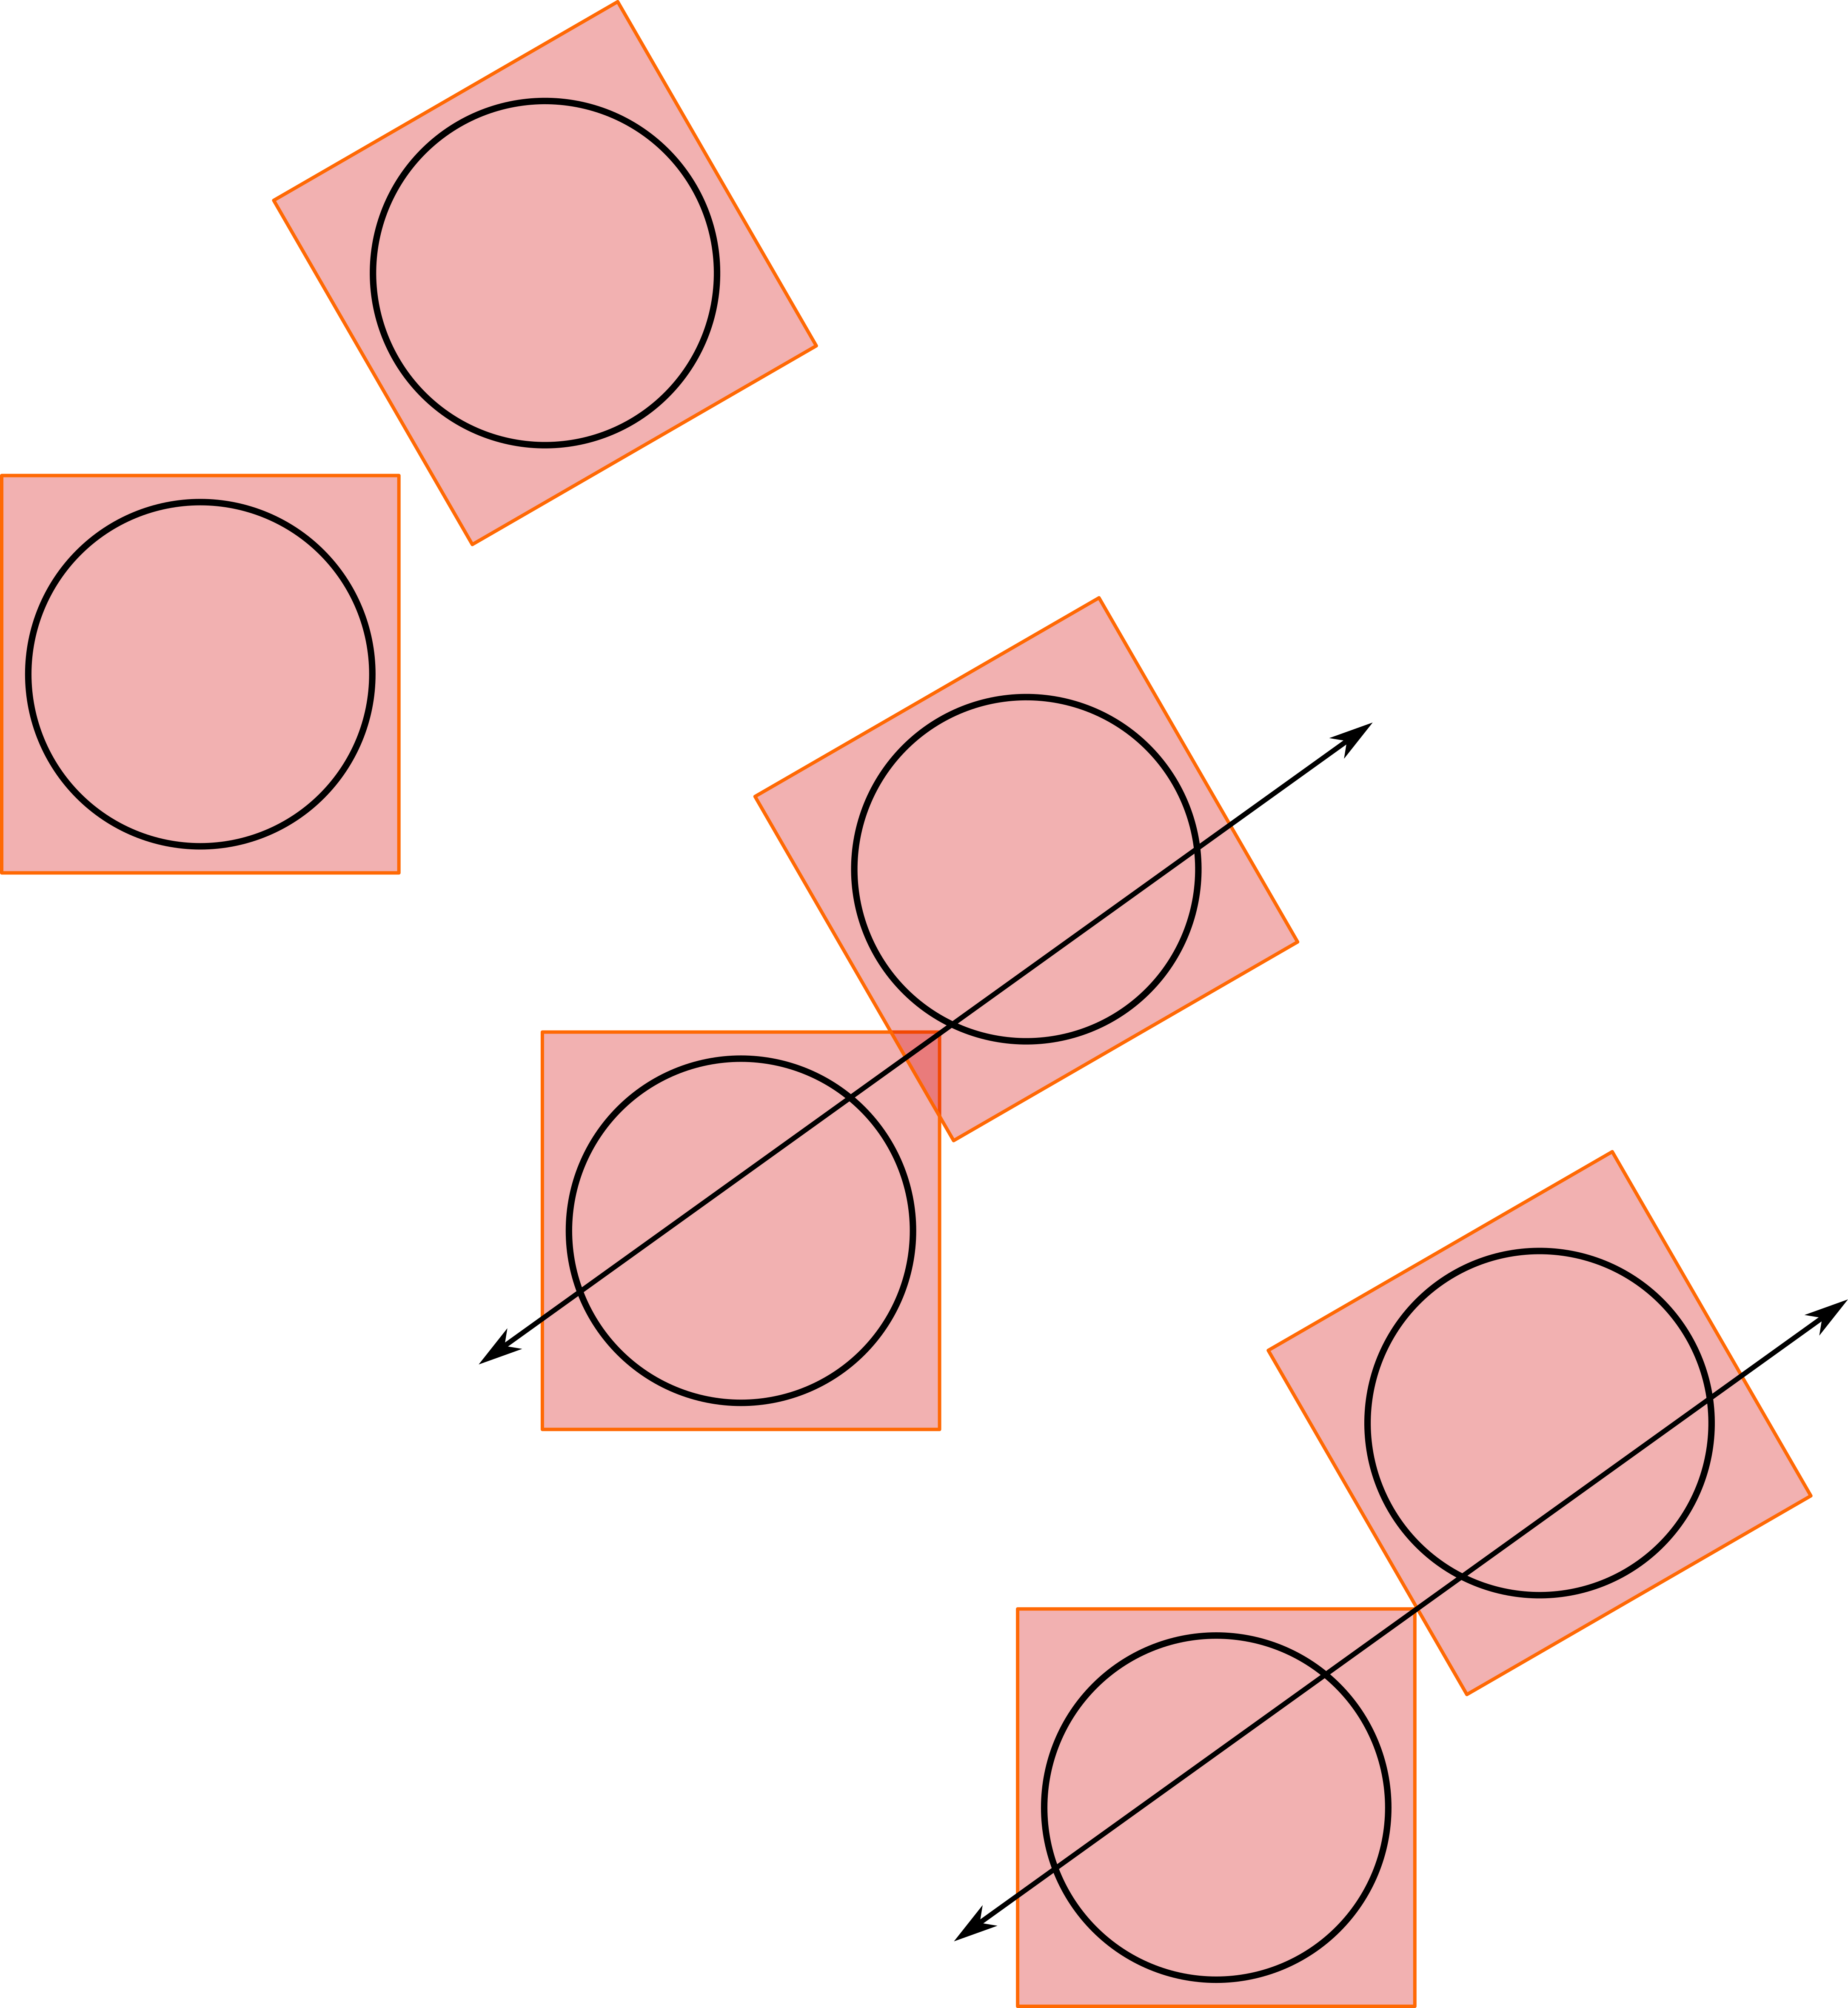
\includegraphics[width = 0.65\textwidth]{./pics/collision_v.png}
      \end{figure}
      \end{column}%
      \begin{column}{0.5\textwidth}
      \begin{itemize}
        \item<1-> Check for collision
        \item<2-> Find collision points
        \item<3-> Check for penetration depth
        \item<4-> Apply force proportional to penetration depth
      \end{itemize}
      \end{column}
    }

    \frame{
      \frametitle{Caveats Collision}

      \begin{itemize}
        \item<1-> Collisions depend strongly on simulation (hyper-) parameters!
        \item<2-> The resulting force are at best a linearization of the real forces!
        \item<3-> Most engines "just" calculate point to point contacts!
        \item<4-> If primitive shapes are used, the behavior is strongly influenced by the shape.
      \end{itemize}
    }

    \frame{
      \frametitle{Friction}
      \begin{figure}
        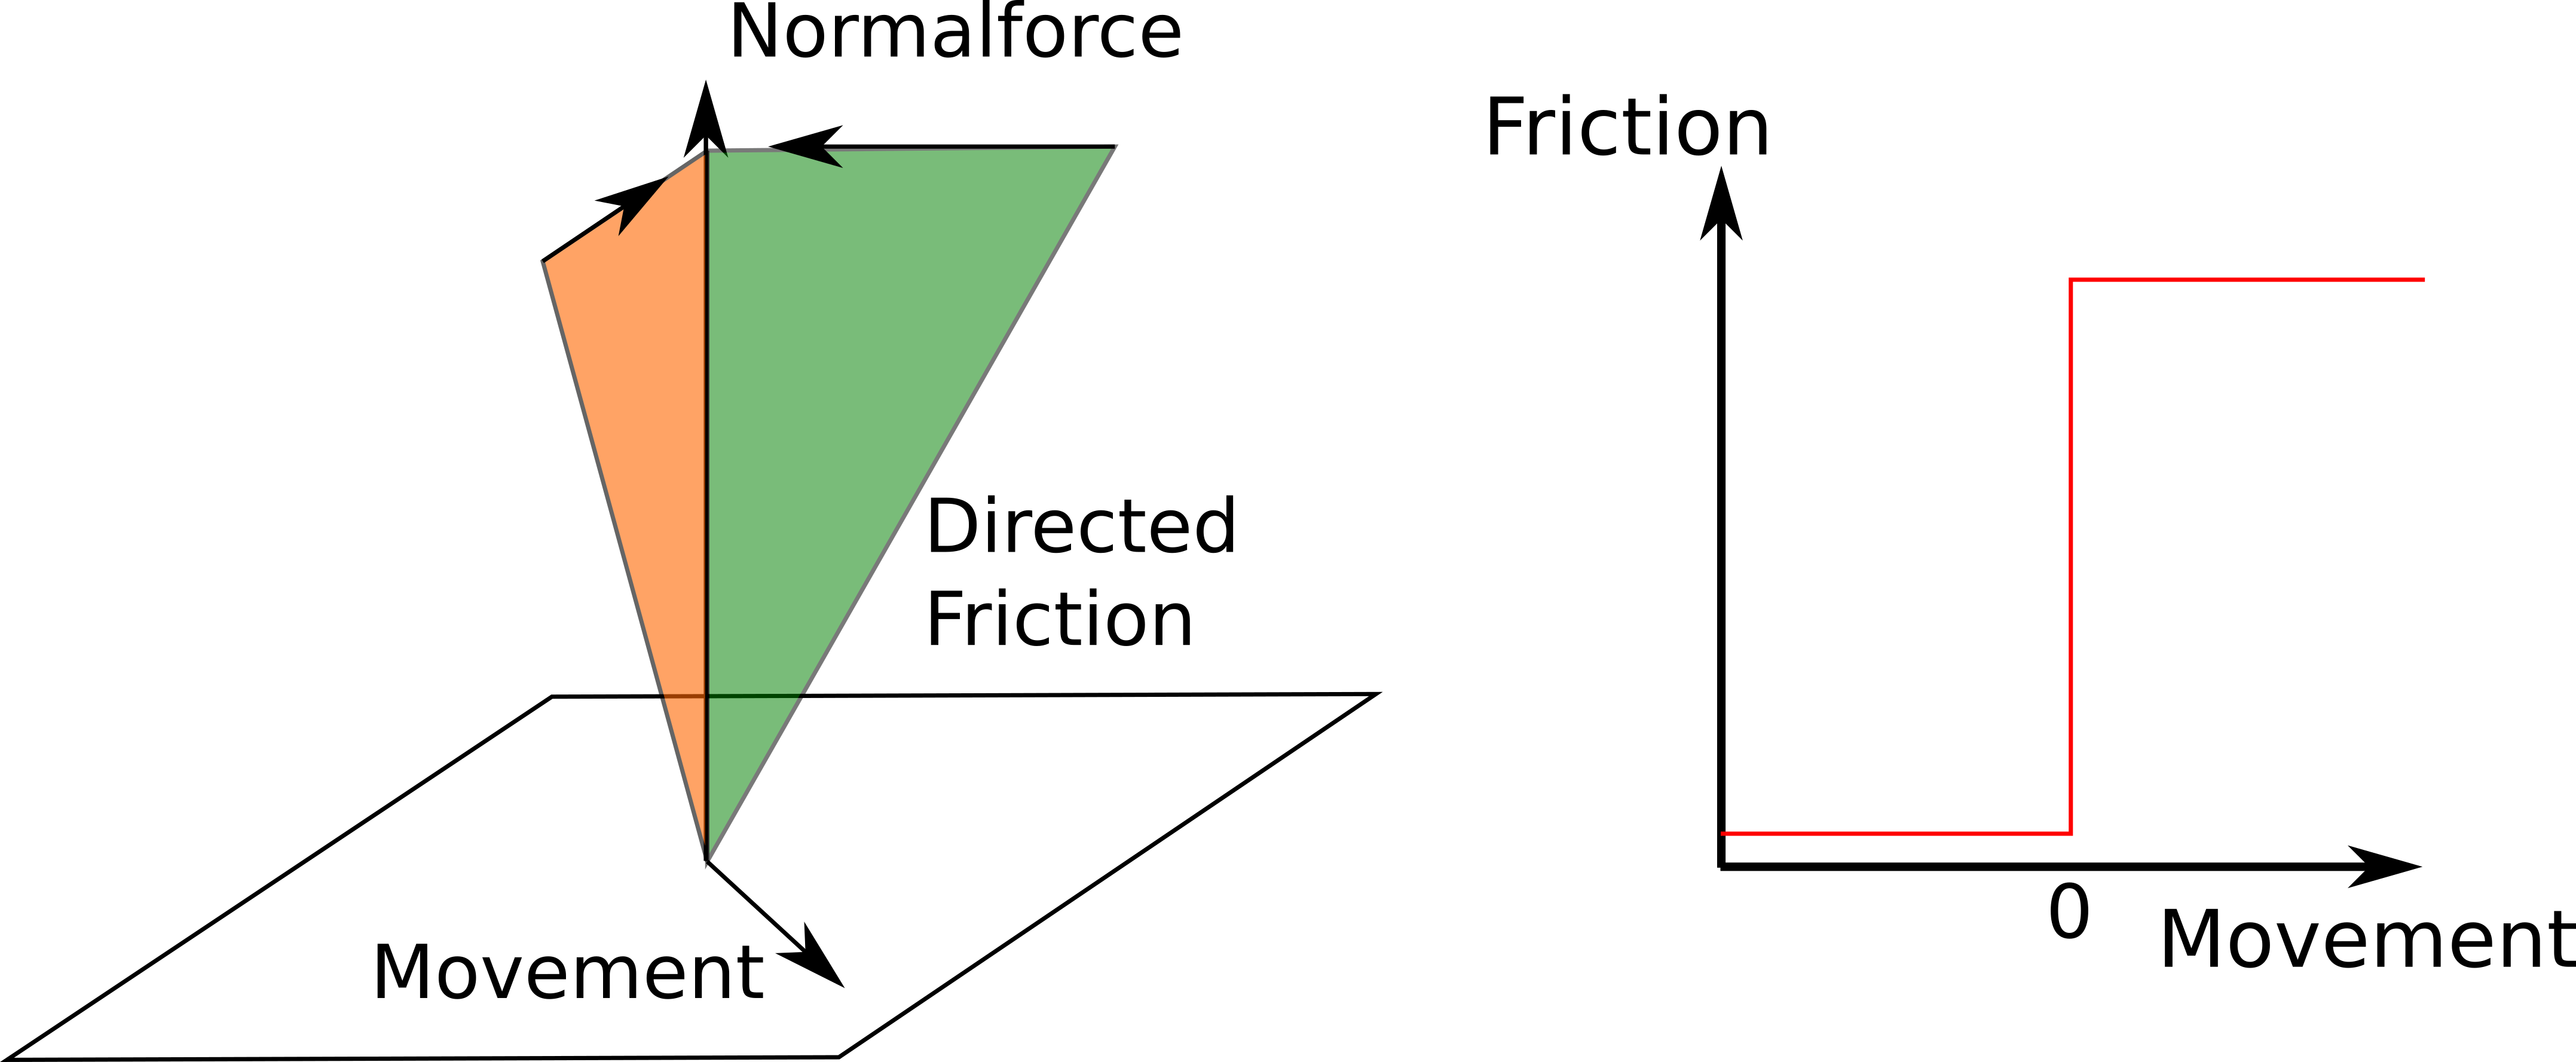
\includegraphics[width = 0.8\textwidth]{./pics/friction.png}
      \end{figure}

    }

    \frame{
      \frametitle{Friction Models}

      Friction in general is described with a simple Coloumb friction model. This model is not sufficient for all use cases!

      \begin{align*}
      Coloumb &: ~F_C = -\mu~F_N  ~sign(\dot{x}) \\
      Viscous &: ~F_V = F_C ~sat(k\dot{x}) \\
      Dankowicz &: ~F_D = \frac{F_{Max}}{\delta}~z \\
                 & ~\dot{z} = \dot{x} \left[ 1- \frac{z}{\delta} ~sign(\dot{x}) \right]
      \end{align*}
    }

    \frame{
      \frametitle{Caveats Friction}

      \begin{itemize}
        \item<1-> Friction is depending on contact force!
        \item<2-> Most likely, only a simple friction model is implemented.
        \item<3-> Sometimes, there is not directional friction.
        \item<4-> If primitive shapes are used, the behavior is strongly influenced by the shape.
      \end{itemize}
    }

    \frame{
      \frametitle{Algorithm for Multibody Dynamics}
      \begin{figure}
        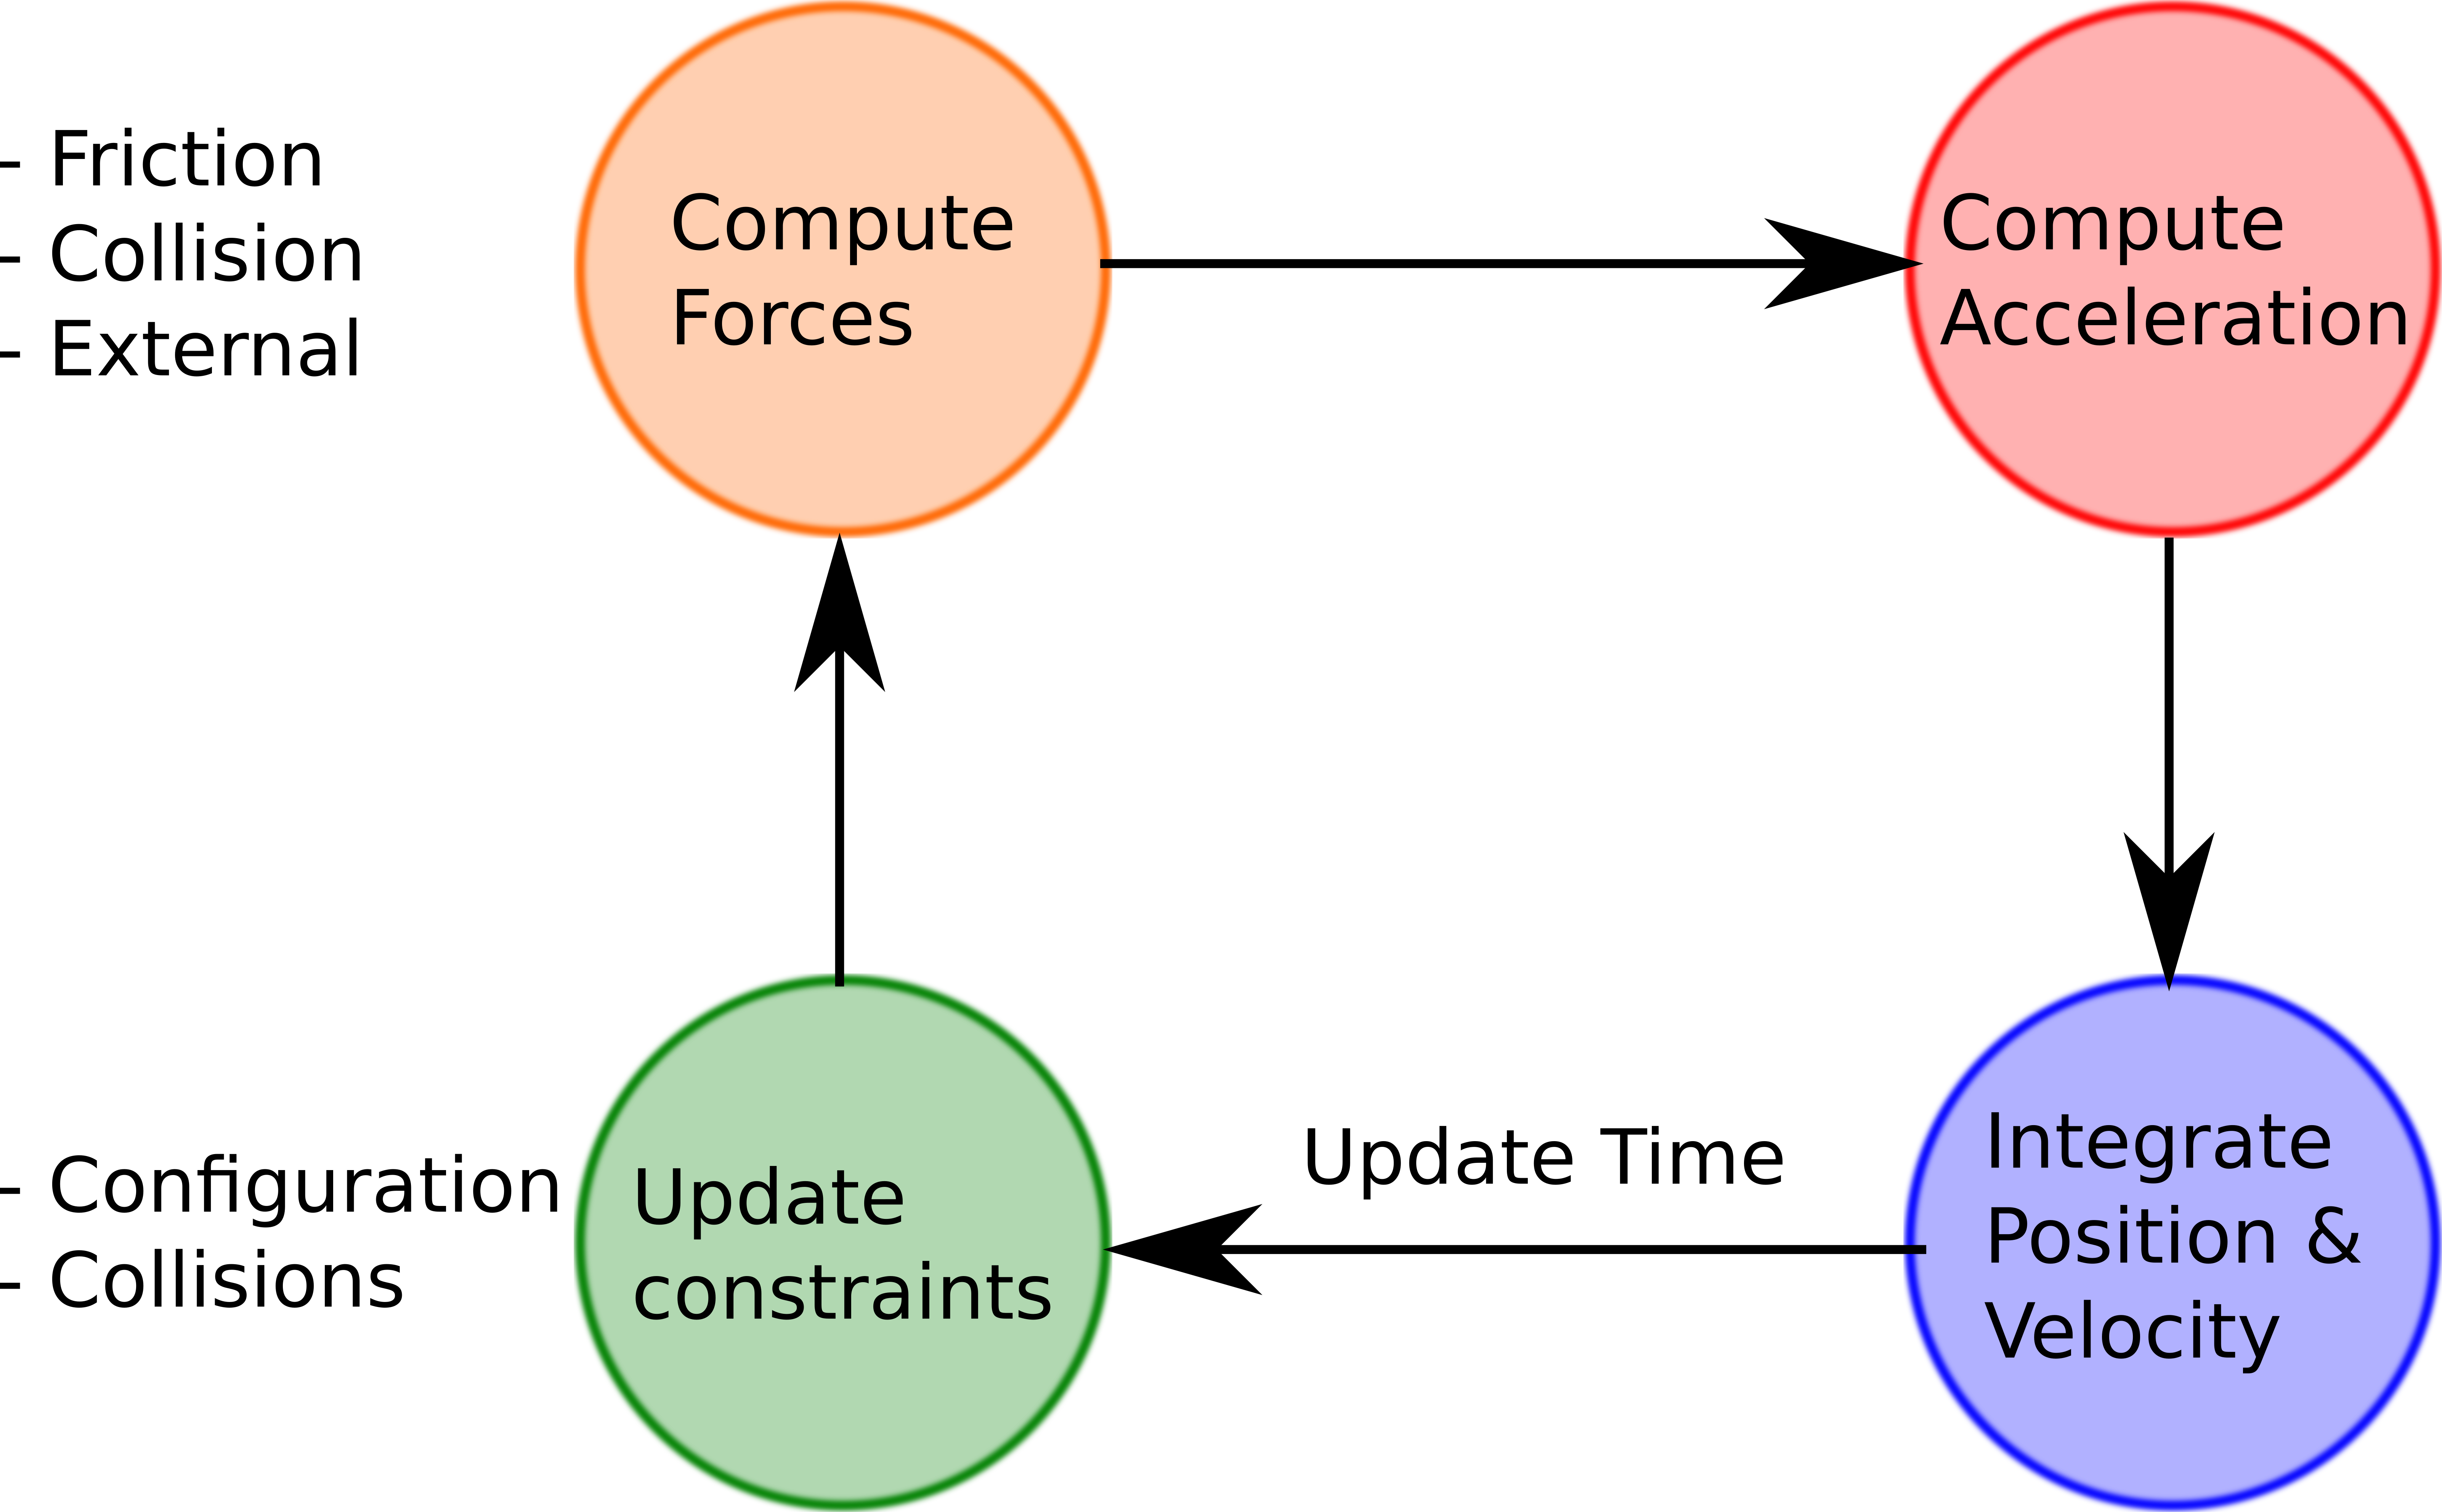
\includegraphics[width = 0.65\textwidth]{./pics/algorithm.png}
      \end{figure}
      %\begin{enumerate}
      %\item Update constraints \\ Compute joint position \\ Check for collision
      %\item Compute external forces \\ Due to constraints \\ Due to collision \\ Due to friction
      %\item Compute acceleration \\ With current configuration
      %\item Integrate numerically \\ Get velocity and position
      %\end{enumerate}
    }

  \section{URDF}

    \frame{
      \frametitle{Universal Robot Description Format}

      \begin{figure}
        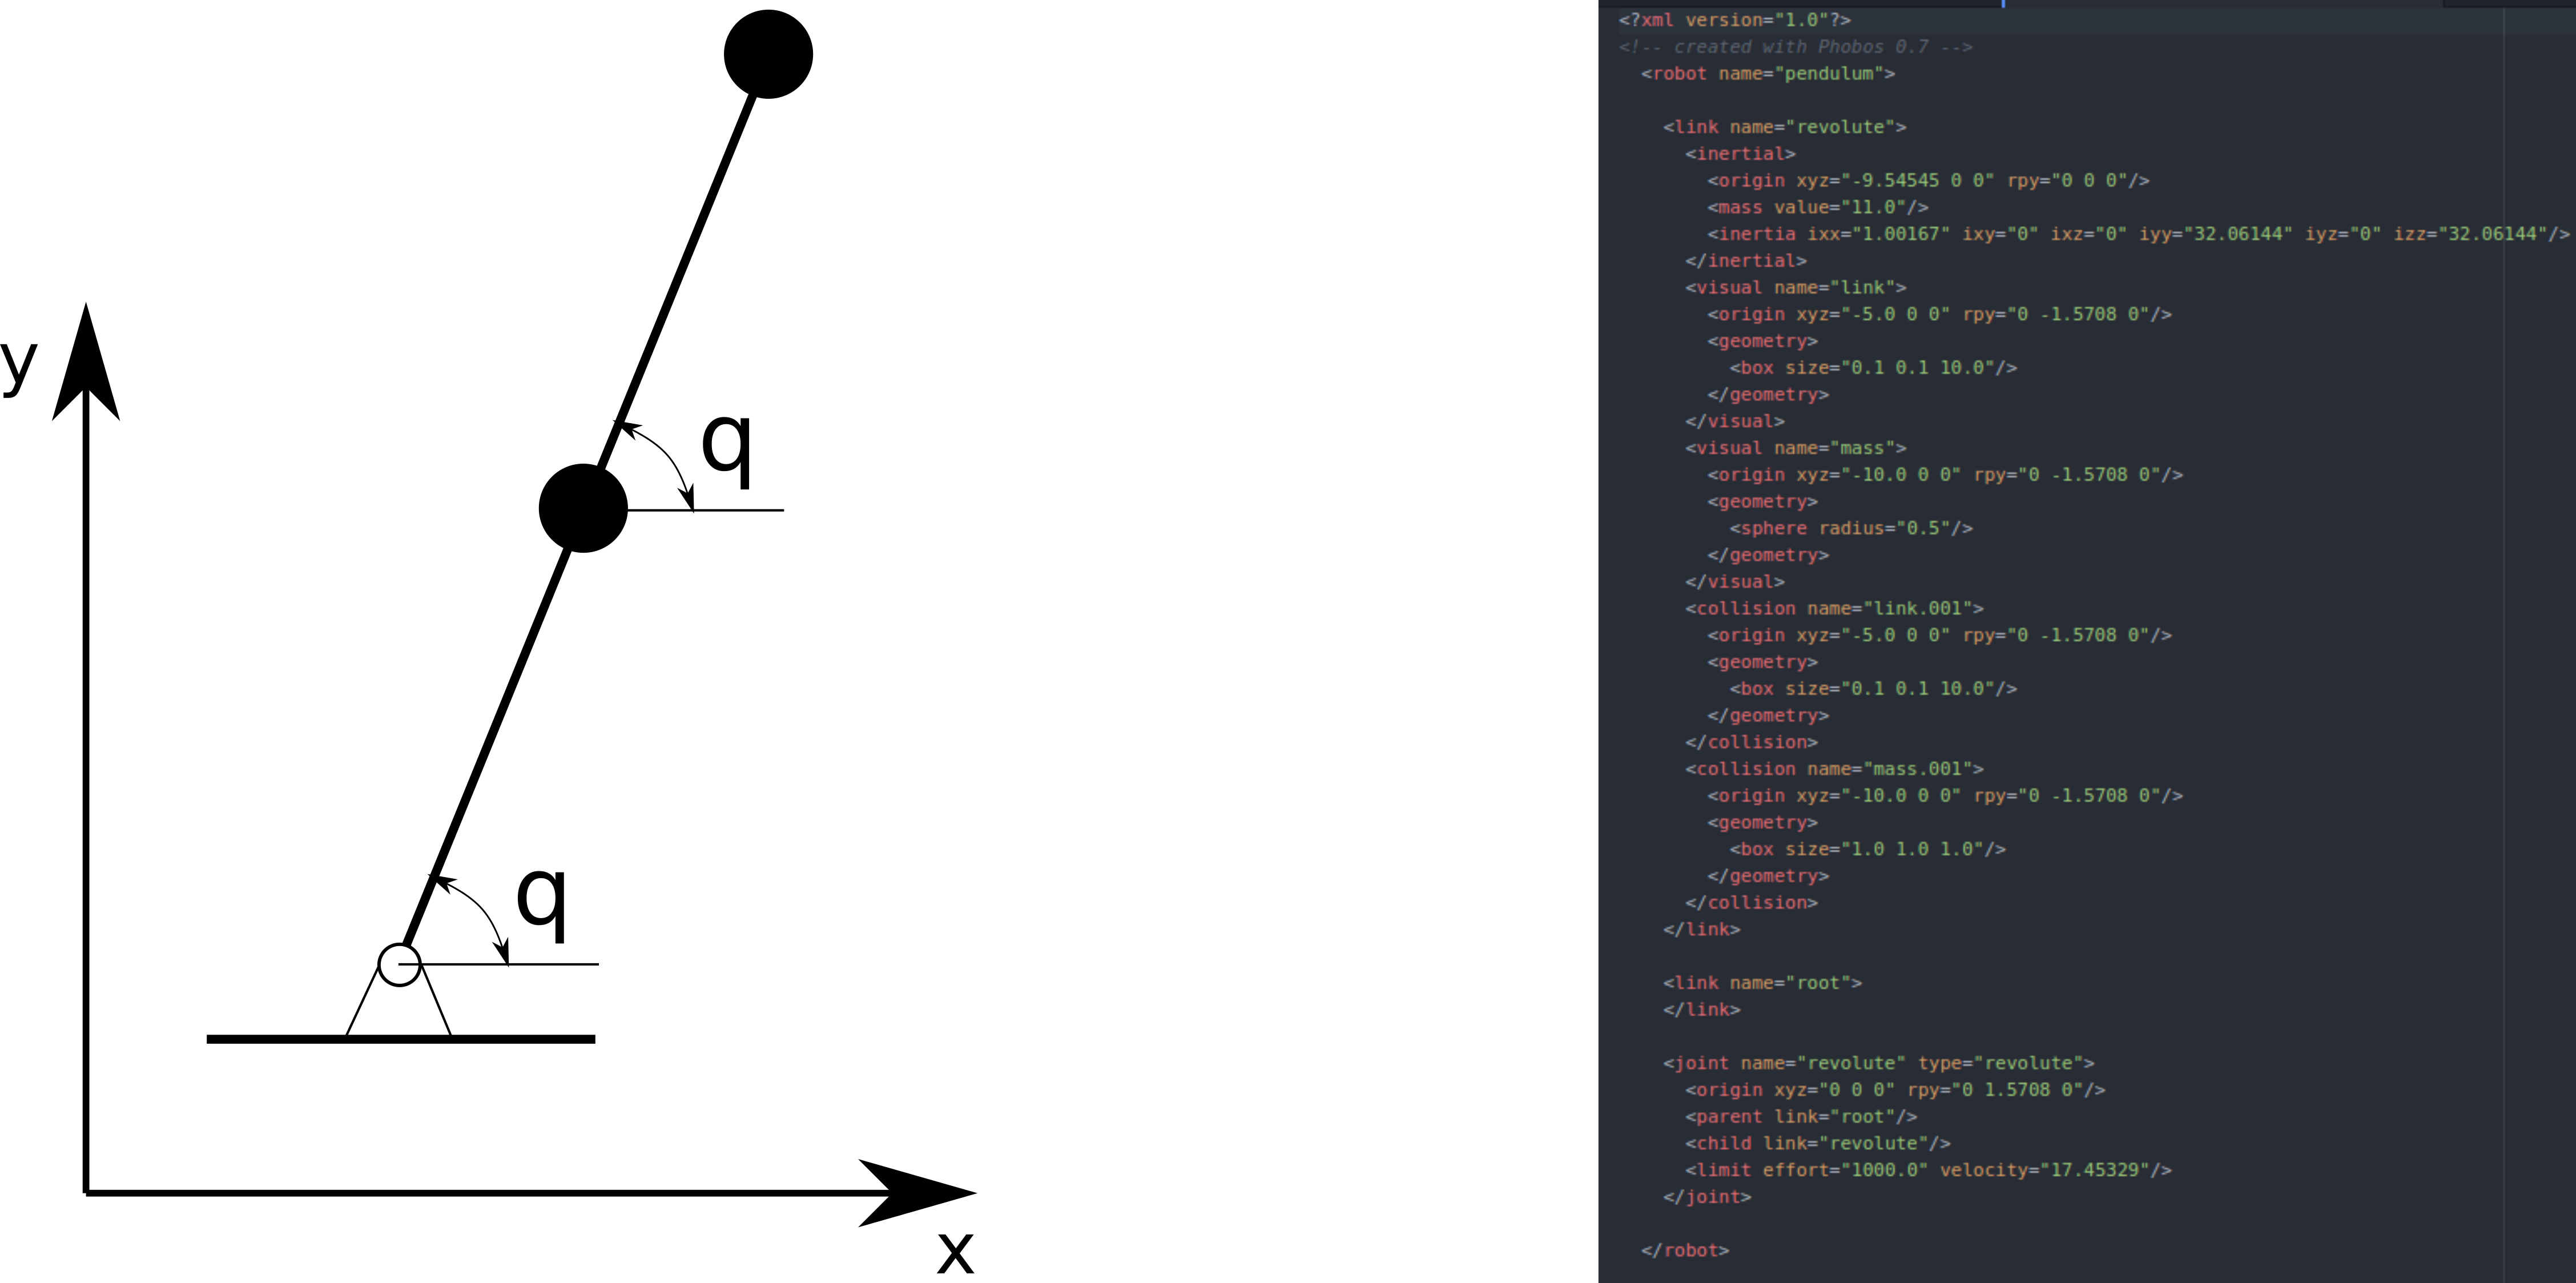
\includegraphics[width = 0.8\textwidth]{./pics/pendulum_to_xml.png}
      \end{figure}

    }


    \frame{
      \frametitle{Links}
      \begin{column}{0.5\textwidth}
      \begin{itemize}
        \item<1-> Name
        \item<2-> Inertial information \\ Mass, Inertia, Pose
        \item<3-> Visual information \\ Origin, Geometry, Pose
        \item<4-> Collision information  \\ Origin. Geometry, Pose
      \end{itemize}
      \end{column}%
      \begin{column}{0.5\textwidth}
      \begin{figure}
        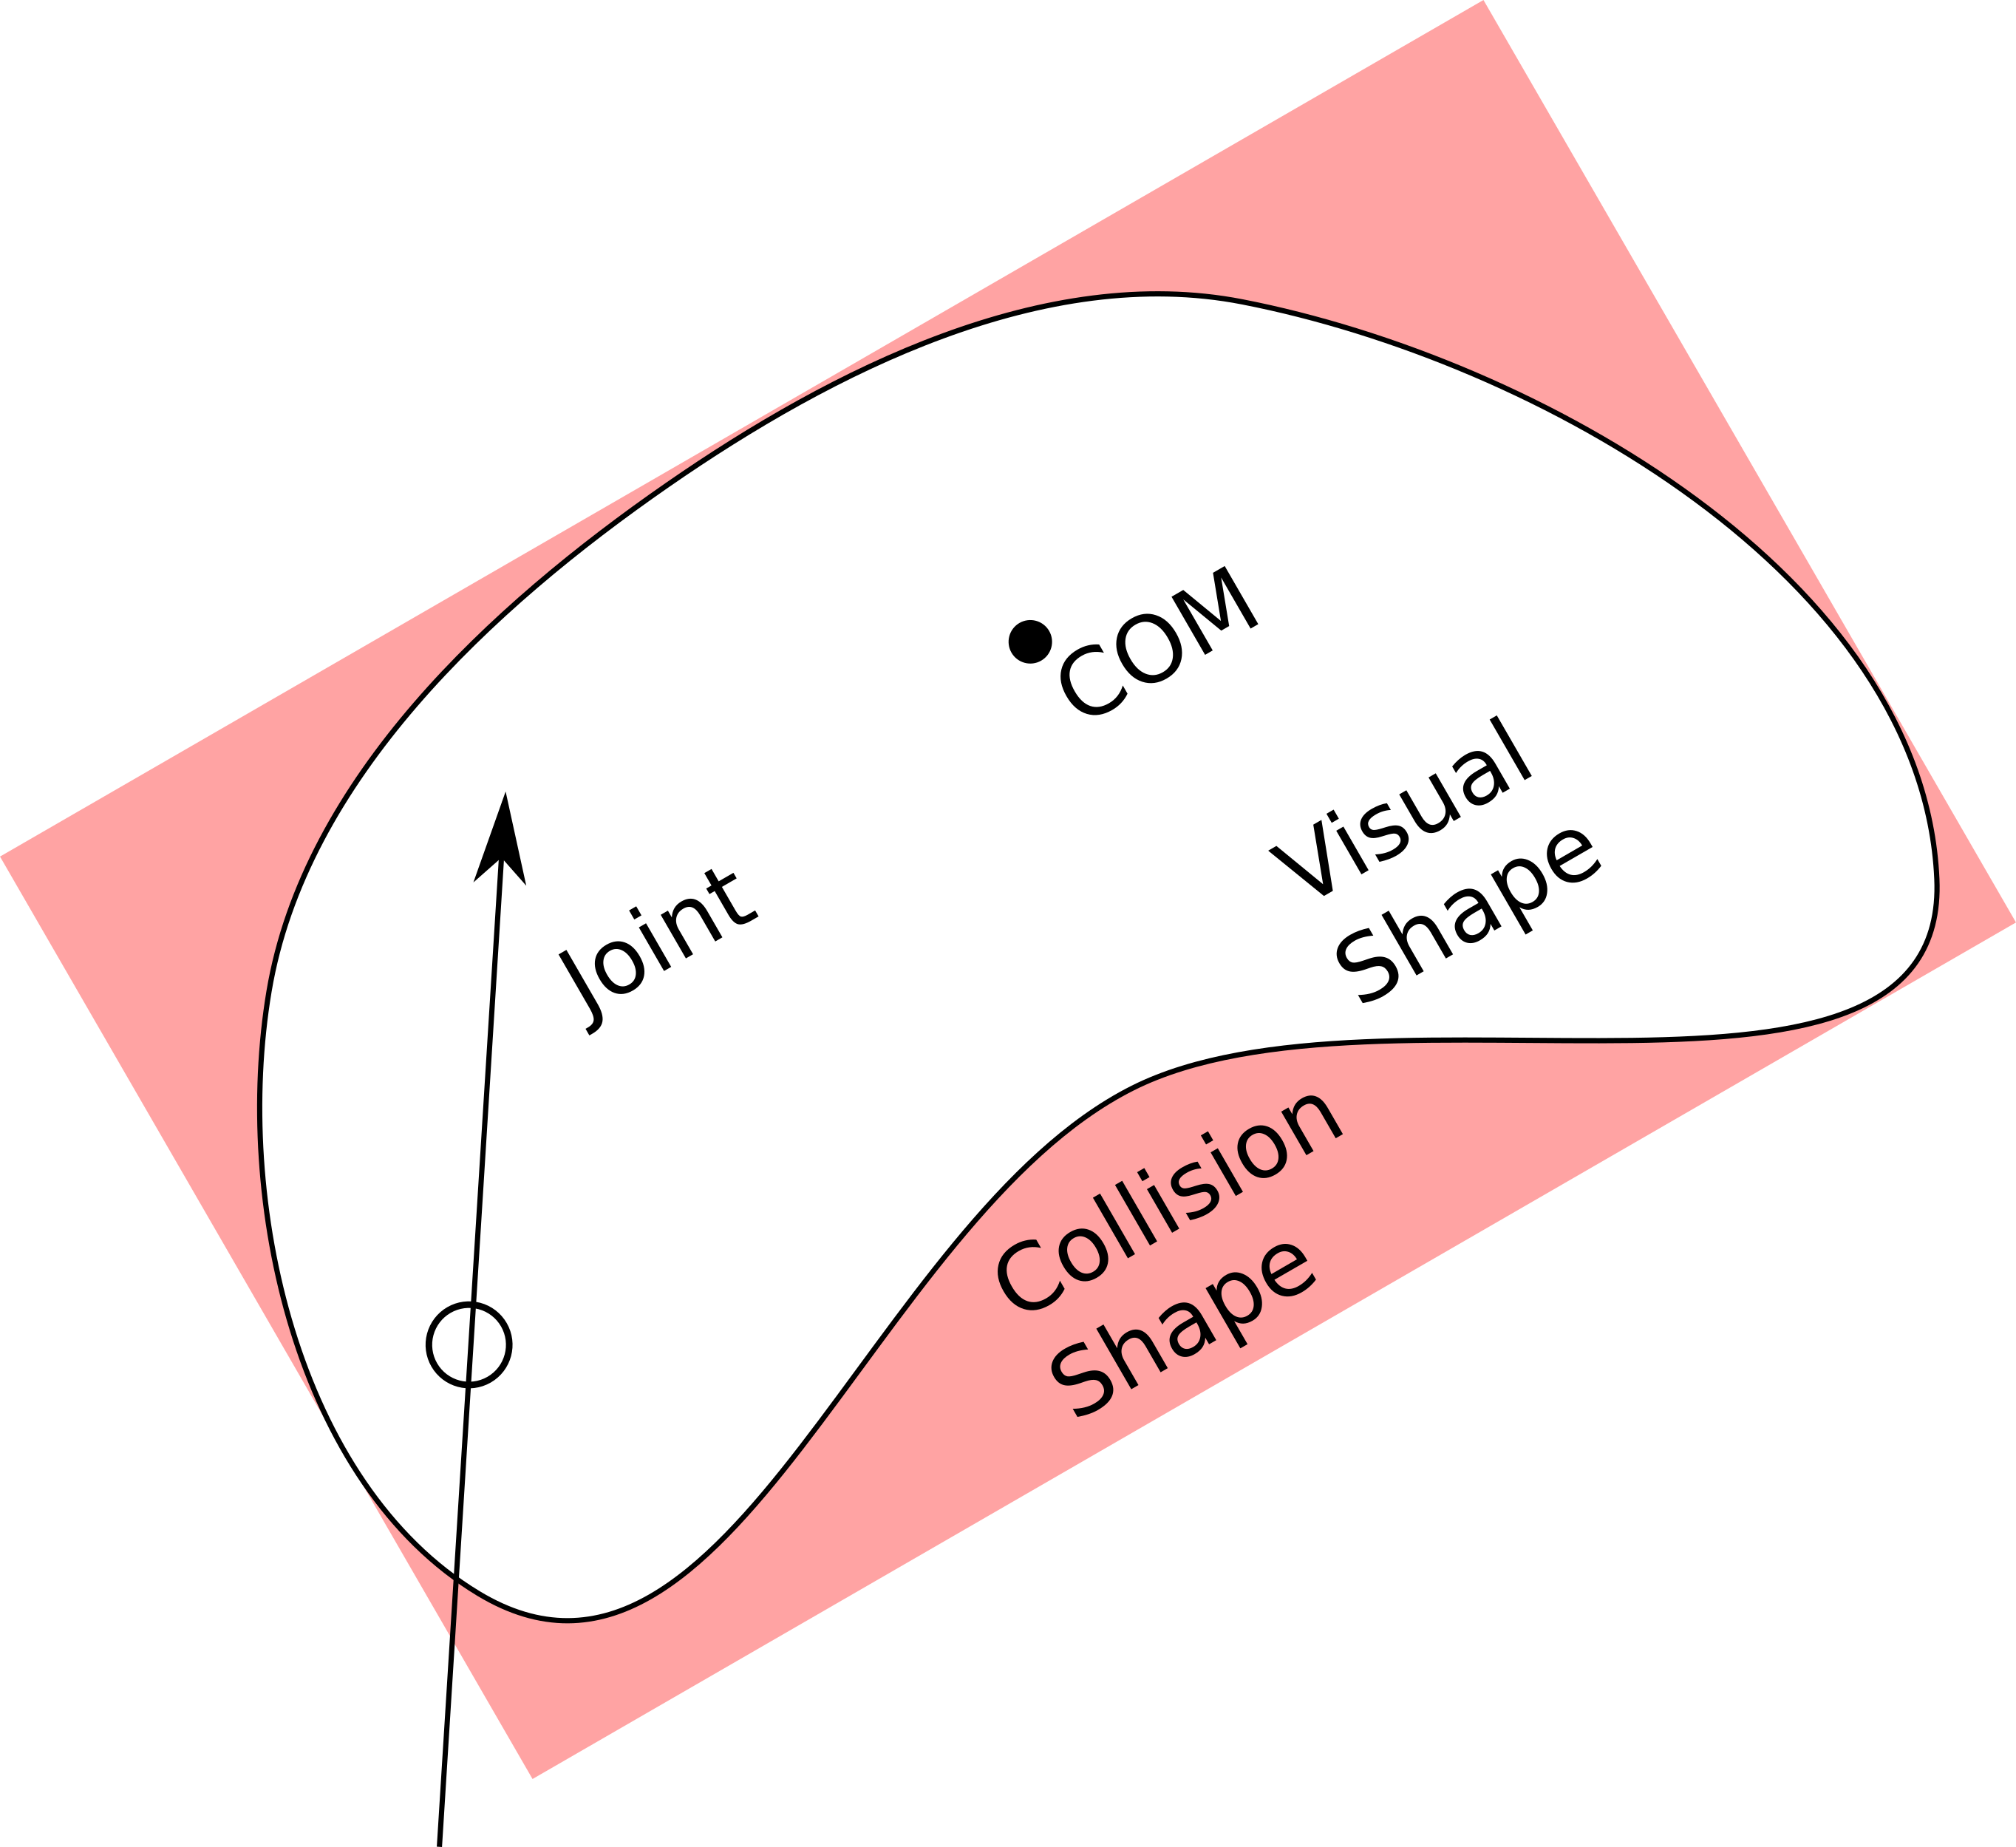
\includegraphics[width = 0.8\textwidth]{./pics/rigid_link.png}
      \end{figure}
      \end{column}

    }

    \frame{
      \frametitle{Joints}
      \begin{column}{0.5\textwidth}
      \begin{itemize}
        \item<1-> Name
        \item<2-> Pose \\ relative to Parent
        \item<3-> Parent Link
        \item<4-> Child Link
        \item<5-> Limits \\ Position, Velocity, Effort
      \end{itemize}
      \end{column}%
      \begin{column}{0.5\textwidth}
      \begin{figure}
        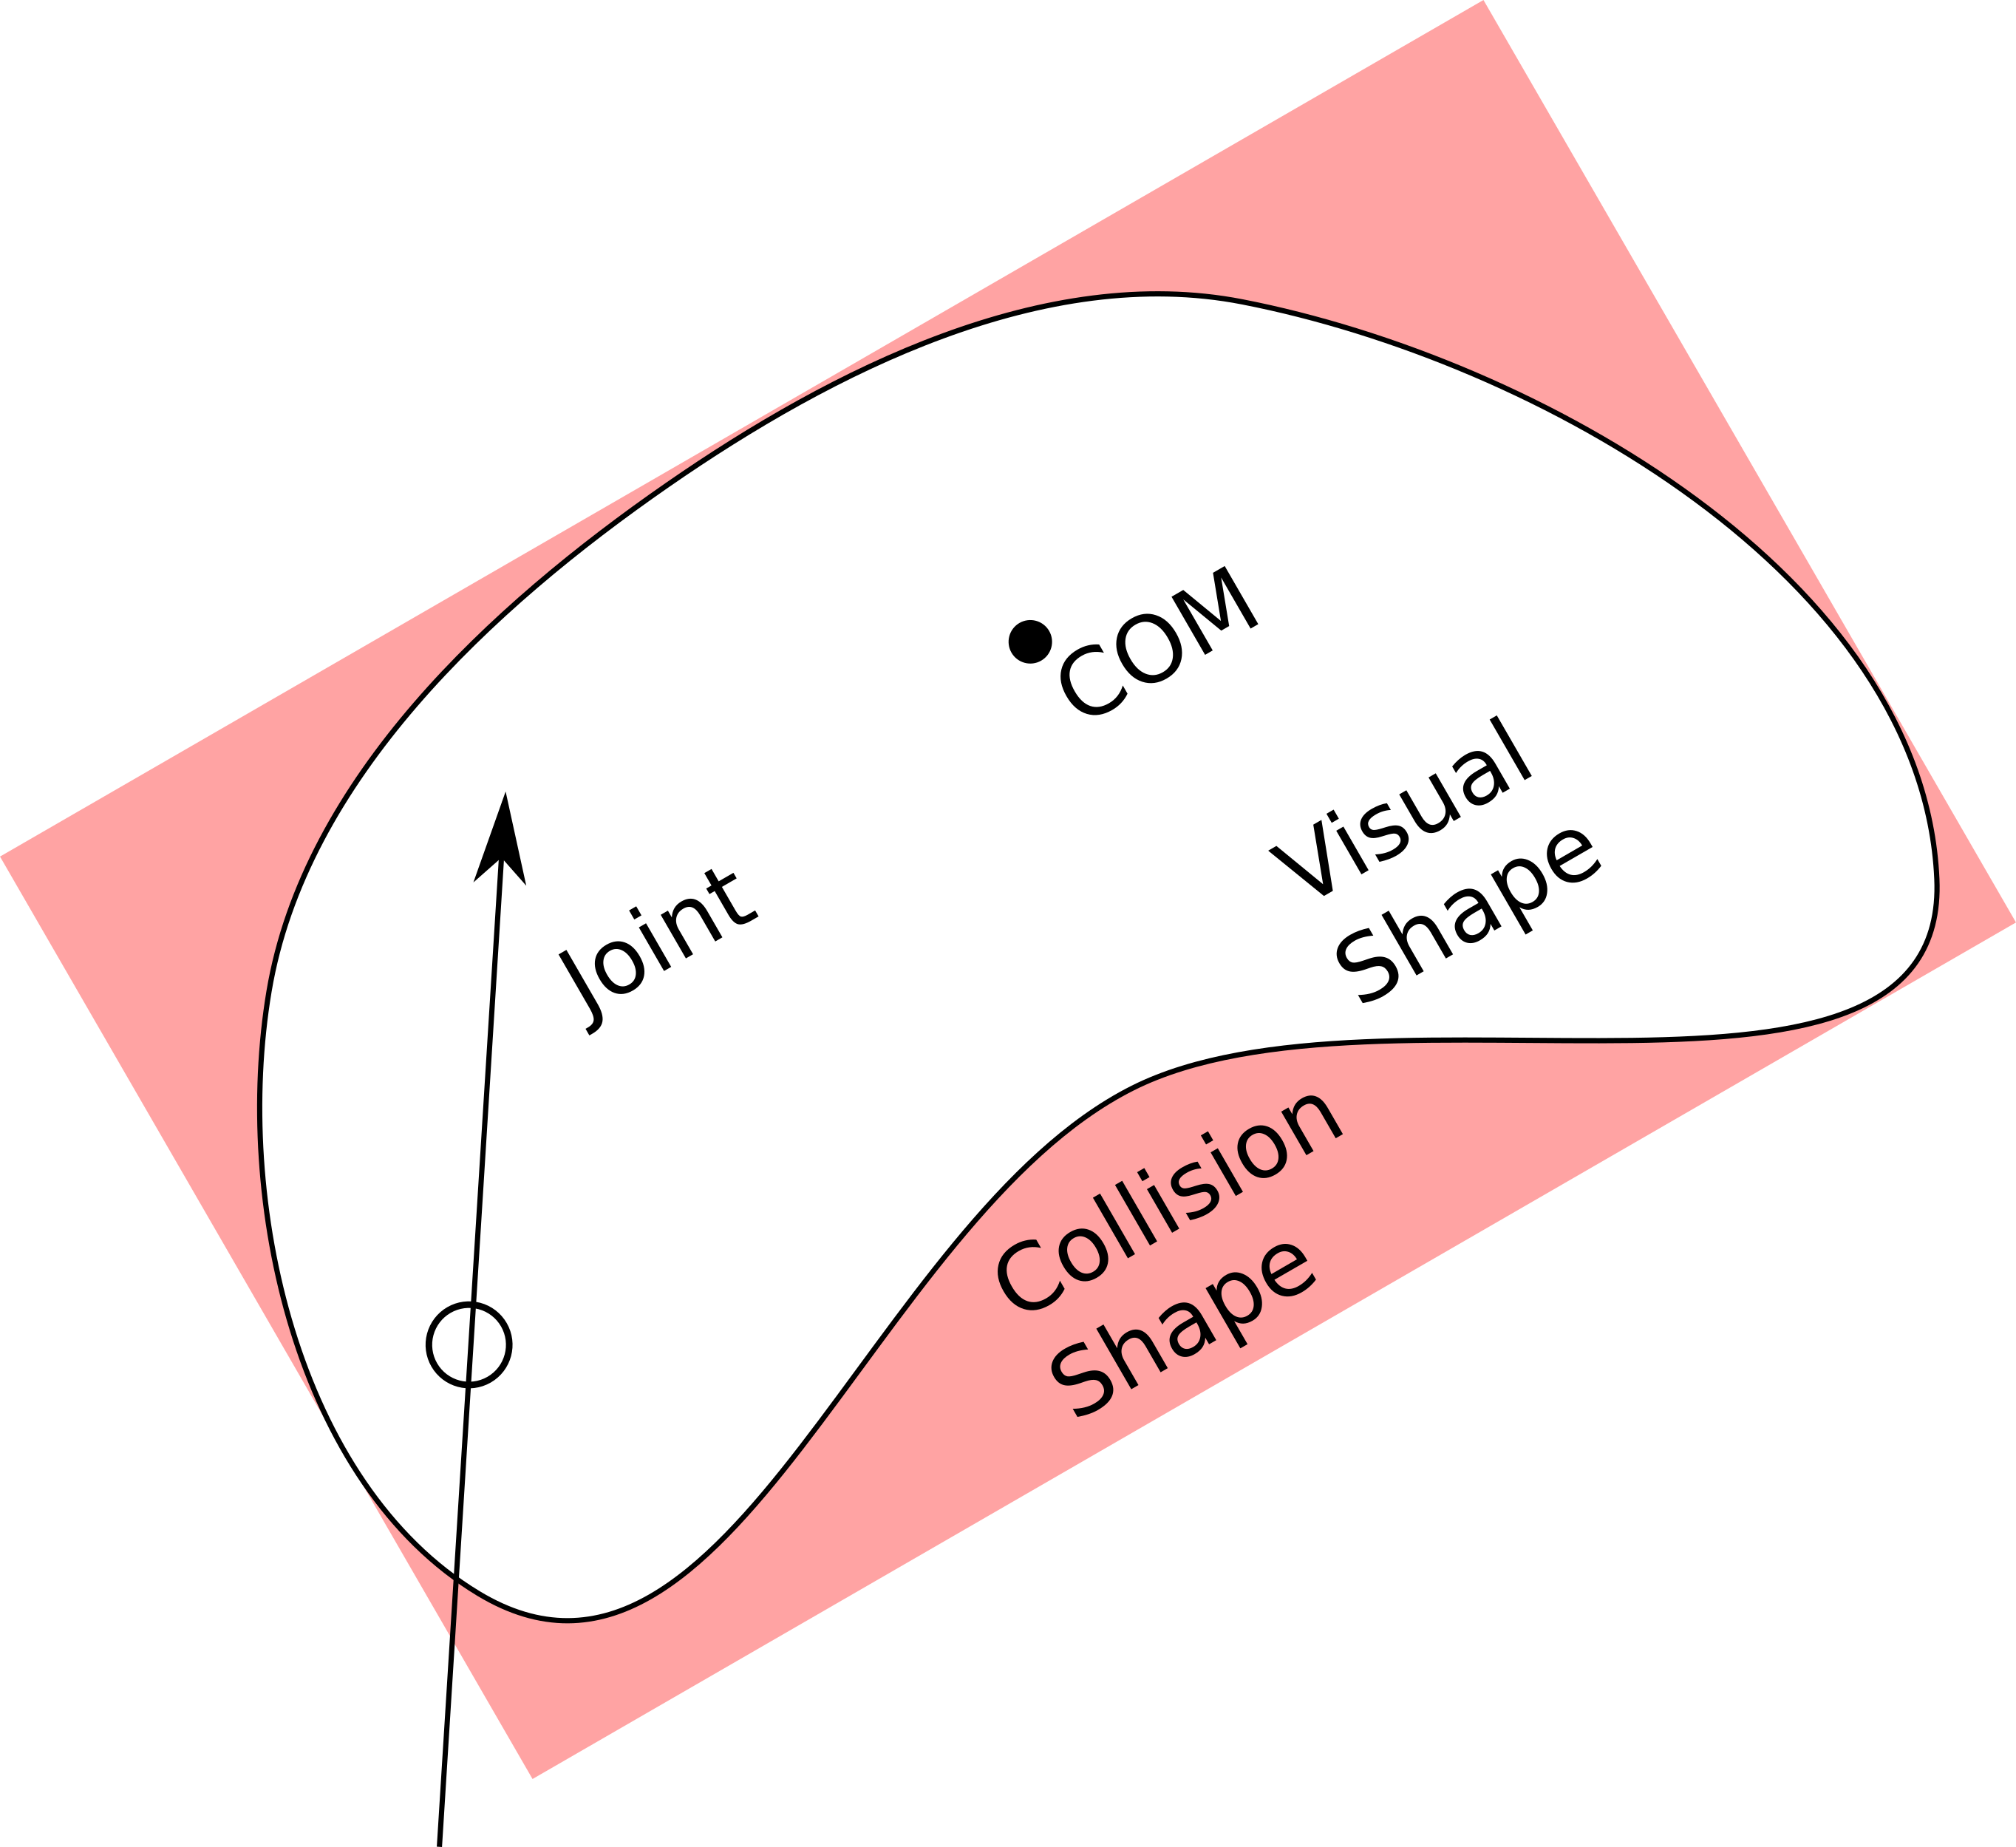
\includegraphics[width = 0.8\textwidth]{./pics/rigid_link.png}
      \end{figure}
      \end{column}

    \frame{
      \frametitle{Phobos - A WYSIWYG Robot Modeling Tool}
      % Maybe put the keyframe into here!?
    }

    }

\end{document}
